\section{The regionally proximal relation}

\begin{frame}
  \begin{definition}[regionally proximal relation]
    \label{def:rpr}
    Let $(X, T)$ be a TDS.
    Two points $x,y \in X$ are called \emph{regionally proximal}
    if and only if for each $\varepsilon > 0$ there exist $x' \in B_\varepsilon(x), y' \in B_\varepsilon(y)$
    and $t \in T$ such that $d(tx', ty') < \varepsilon$.
    We denote the set of regionally proximal pairs by $Q_2(X) \subseteq X \times X$.
  \end{definition}
  \begin{tikzpicture}[scale = 1.4]
  % Coordinates of the main points
  \coordinate (A) at (2,3);
  \coordinate (B) at (2.5,1.5);

  % Off-center lighter points initial positions
  \coordinate (Alight) at ($(A) + (5pt,2pt)$);
  \coordinate (Blight) at ($(B) + (-5pt,-2pt)$);

  % Midpoint of lighter points
  \coordinate (Mid) at ($0.5*(Alight) + 0.5*(Blight)$);

  % Meeting point shifted 2 cm to the right of Mid
  \coordinate (M) at ($(Mid) + (2cm,0)$);

  % Draw dotted circles around main points
  \draw[dotted, thick] (A) circle (10pt);
  \draw[dotted, thick] (B) circle (10pt);

  \node[red, above left] at (A) {$x$};
  \node[blue, below right] at (B) {$y$};

  % Draw main points (smaller)
  \fill[red] (A) circle (2pt);
  \fill[blue] (B) circle (2pt);

  % Draw lighter points at initial positions
  \fill[red!50] (Alight) circle (1.5pt);
  \fill[blue!50] (Blight) circle (1.5pt);

  \node[red!50, above right] at (Alight) {$x'$};
  \node[blue!50, below left] at (Blight) {$y'$};

  % Draw trajectories of lighter points toward the meeting point
  \draw[red!50, thick, ->] (Alight) to[out=0,in=145] ($(M) + (0, 0.2)$);
  \draw[blue!50, thick, ->] (Blight) to[out=0,in=-145] (M);

  % Draw meeting point
  \draw[dotted, thick] (M) circle (10pt);

  \node[red!50, above right] at (M) {$tx'$};
  \node[blue!50, below right] at (M) {$ty'$};

\end{tikzpicture}
\end{frame}

\begin{frame}
  Example of regionally proximal pair $(0, 1)$ with the system \ref{}:
  \include{tikz/rpr-ex1}
  with $t$ large enough:
  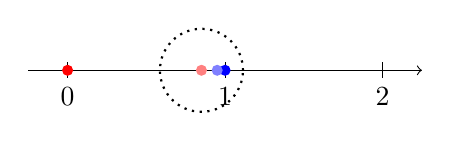
\begin{tikzpicture}
  \draw[->] (-0.5,0) -- (4.5,0) node[right] {};
  
  % Draw ticks and labels
  \foreach \x in {0,1,2} {
    \draw (2*\x,0.1) -- (2*\x,-0.1) node[below] {\x};
  }

  \fill[red] (0,0) circle (2pt);
  \fill[red!50] (1.7,0) circle (2pt);

  \fill[blue] (2,0) circle (2pt);
  \fill[blue!50] (1.9,0) circle (2pt);

  \draw[thick, dotted] (1.7,0) circle (15pt);
\end{tikzpicture}
\end{frame}